%%=============================================================================
%% Inleiding
%%=============================================================================

\chapter{\IfLanguageName{dutch}{Inleiding}{Introduction}}%
\label{ch:inleiding}

De inleiding moet de lezer net genoeg informatie verschaffen om het onderwerp te begrijpen en in te zien waarom de onderzoeksvraag de moeite waard is om te onderzoeken. In de inleiding ga je literatuurverwijzingen beperken, zodat de tekst vlot leesbaar blijft. Je kan de inleiding verder onderverdelen in secties als dit de tekst verduidelijkt. Zaken die aan bod kunnen komen in de inleiding~\autocite{Pollefliet2011}:

\begin{itemize}
  \item context, achtergrond
  \item afbakenen van het onderwerp
  \item verantwoording van het onderwerp, methodologie
  \item probleemstelling
  \item onderzoeksdoelstelling
  \item onderzoeksvraag
  \item \ldots
\end{itemize}

\section{\IfLanguageName{dutch}{Probleemstelling}{Problem Statement}}%
\label{sec:probleemstelling}

%Uit je probleemstelling moet duidelijk zijn dat je onderzoek een meerwaarde heeft voor een concrete doelgroep. De doelgroep moet goed gedefinieerd en afgelijnd zijn. Doelgroepen als ``bedrijven,'' ``KMO's'', systeembeheerders, enz.~zijn nog te vaag. Als je een lijstje kan maken van de personen/organisaties die een meerwaarde zullen vinden in deze bachelorproef (dit is eigenlijk je steekproefkader), dan is dat een indicatie dat de doelgroep goed gedefinieerd is. Dit kan een enkel bedrijf zijn of zelfs één persoon (je co-promotor/opdrachtgever). \\

Anderhalf miljoen elektrische wagens, massaal veel warmtepompen en zonnepanelen gecombineerd met een toenemende elektrificatie van de industrie en het vrachtvervoer tegen 2030. Dat is de verwachting van de Vlaamse distributienetbeheerder Fluvius \autocite{Verdoodt2022}. De energietransitie die vanuit Europa, België en Vlaanderen wordt aangestuurd, vormt een enorme uitdaging voor de distributienetten voor elektriciteit in Vlaanderen. \\

\begin{figure}
    \centering\includegraphics[scale=0.4]{Elektrificatie_personenvoertuigen}
    \caption{\label{fig:Aantal_el_personenvoertuigen}Verwachte evolutie van het aantal
        elektrische personenvoertuigen in Vlaanderen \autocite{Verdoodt2022}.}
\end{figure}

\begin{figure}
    \centering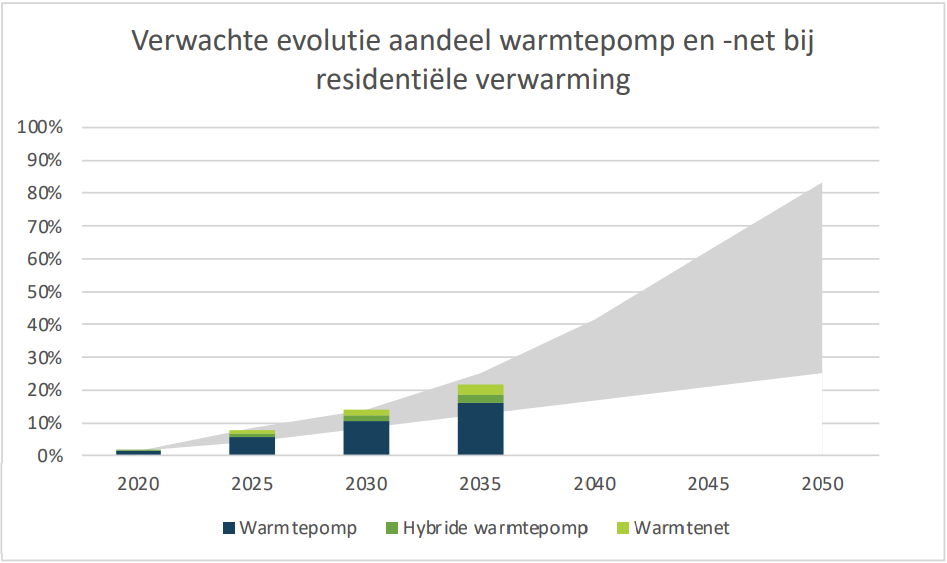
\includegraphics[scale=0.4]{Evolutie_Warmtepomp}
    \caption{\label{fig:Evolutie_Warmtepompen}Verwachte evolutie van het aandeel warmtepomp en -net bij
        residentiële verwarming in Vlaanderen \autocite{Verdoodt2022}.}
\end{figure}

\begin{figure}
    \centering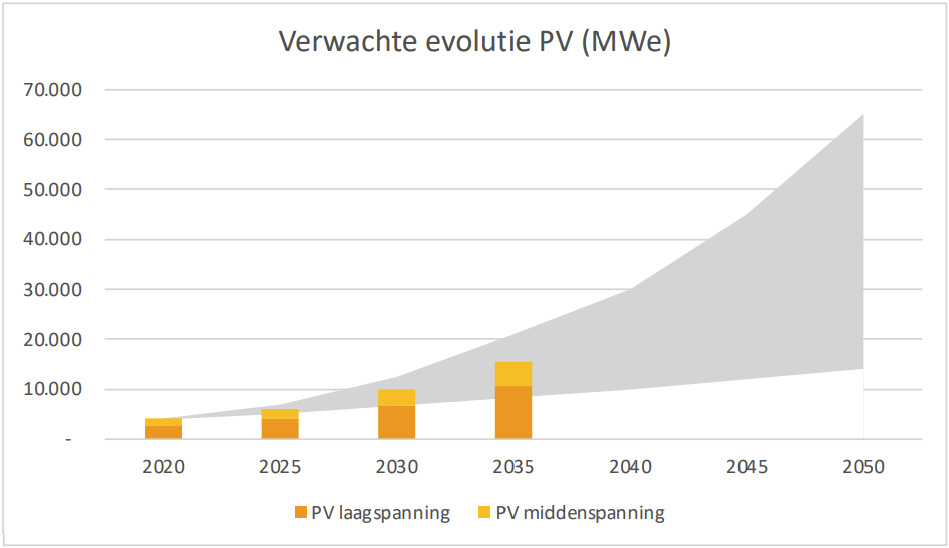
\includegraphics[scale=0.4]{Evolutie_PV}
    \caption{\label{fig:Evolutie_PV}Verwachte evolutie van zonnepanelen in Vlaanderen \autocite{Verdoodt2022}.}
\end{figure}

\begin{figure}
    \centering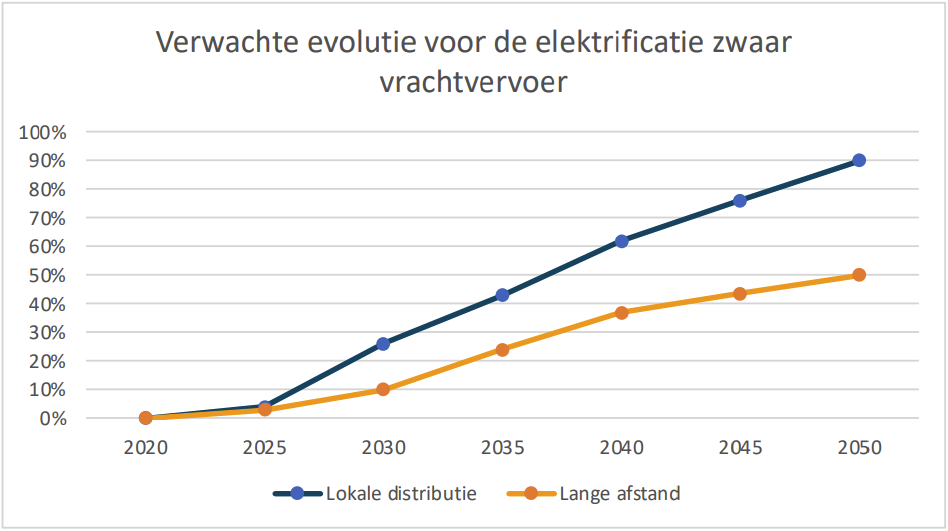
\includegraphics[scale=0.4]{Elektrificatie_Vrachtvervoer}
    \caption{\label{fig:El_Vrachtvervoer}Verwachte evolutie van de elektrificatie van zwaar
        vrachtvervoer in Vlaanderen \autocite{Verdoodt2022}.}
\end{figure}

Om al te hoge investeringen in de distributienetten te vermijden, wordt door Fluvius ingezet op maatregelen die de belasting van het elektriciteitsnet kunnen verminderen en spreiden. Een van die maatregelen is de invoering en verplichting van de digitale elektriciteitsmeter. Tegen juli 2029 moeten alle Belgische huishoudens een digitale meter hebben. Deze digitale meters kunnen via een dongle en een app 'slimmer' gemaakt worden, zodat gezinnen hun elektriciteitsverbruik in detail kunnen opvolgen en bijsturen. Dit zal dan meteen ook een besparing voor hen opleveren. Deze apps vereisen echter steeds een actieve opvolging van de gebruiker. Uit onderzoek is gebleken dat deze actieve bijsturing na verloop van tijd vermindert \autocite{Wemyss2019}. Een enquête van de Vlaamse Regulator van de Elektriciteits- en Gasmarkt \textcite{VREG2021} waarin 1.000 Vlaamse gezinnen en 1.500 bedrijven bevraagd werden over hun ervaring en gedrag op de energiemarkt toont zelfs aan dat van de 60\% van de gezinnen met een digitale meter, slechts 8\% hun energieverbruik effectief bijstuurt. Door de invoering van het capaciteitstarief, een andere maatregel waarmee de VREG het elektriciteitsnet hoopt te ontlasten, zal de bijsturing en vooral spreiding van het elektriciteitsverbruik nog belangrijker worden voor gezinnen. Sinds 1 januari 2023 wordt immers een deel van de nettarieven die een gezin via haar elektriciteitsfactuur betaalt ook berekend op het maximale elektriciteitsverbruik. Er wordt dus voortaan ook gekeken naar de maximale capaciteit die de distributienetbeheerders ter beschikking moeten stellen. Bedoeling van het capaciteitstarief is dat gezinnen hun stroomverbruik beter gaan spreiden. Als iedereen op hetzelfde moment veel stroom verbruikt, kan het net overbelast raken. Het gevolg is dat netbedrijven dan extra moeten investeren in zwaardere elektriciteitskabels om die hogere verbruikspieken op te vangen \autocite{Selleslagh2022}. \\

Daarom wordt binnen Fluvius de vraag gesteld hoe nieuwe technologieën en technieken een oplossing kunnen bieden om gezinnen te helpen bij het spreiden van hun elektriciteitsverbruik. Kunnen apps die het elektriciteitsverbuik monitoren slimmer gemaakt worden zodat ze geen tussenkomst van een gebruiker meer behoeven? Kan bijvoorbeeld artificiële intelligentie (AI) daarbij een oplossing bieden? Om dit na te gaan, zal tijdens dit onderzoek een app ontwikkeld worden die het elektriciteitsverbruik zal aansturen op basis van weersvoorspellingen en historische verbruiksdata.

\section{\IfLanguageName{dutch}{Onderzoeksvraag}{Research question}}%
\label{sec:onderzoeksvraag}

%Wees zo concreet mogelijk bij het formuleren van je onderzoeksvraag. Een onderzoeksvraag is trouwens iets waar nog niemand op dit moment een antwoord heeft (voor zover je kan nagaan). Het opzoeken van bestaande informatie (bv. ``welke tools bestaan er voor deze toepassing?'') is dus geen onderzoeksvraag. Je kan de onderzoeksvraag verder specifiëren in deelvragen. Bv.~als je onderzoek gaat over performantiemetingen, dan 

Kan het elektriciteitsverbruik van gezinnen automatisch bijgestuurd en gespreid worden met behulp van artificiële intelligentie om zo de elektriciteitskost te drukken? \\

Kan een app die het elektriciteitsverbruik en de door zonnepanelen geproduceerde elektriciteit meet en voorspelt ervoor zorgen dat het toekomstige elektriciteitsverbruik beter wordt afgestemd op de zelf geproduceerde stroom?

\section{\IfLanguageName{dutch}{Onderzoeksdoelstelling}{Research objective}}%
\label{sec:onderzoeksdoelstelling}

%Wat is het beoogde resultaat van je bachelorproef? Wat zijn de criteria voor succes? Beschrijf die zo concreet mogelijk. Gaat het bv.\ om een proof-of-concept, een prototype, een verslag met aanbevelingen, een vergelijkende studie, enz.

Om na te gaan of het elektriciteitsverbruik van een gezin automatisch kan gestuurd en gespreid worden, zal een app ontwikkeld worden die in de eerste plaats het elektriciteitsverbruik en de zelf geproduceerde stroom van zonnepanelen inzichtelijk maakt. De gemeten gegevens zullen daarna samen met de weerdata van een weer API gebruikt worden om met artificiële intelligentie een voorspelling van de elektriciteitsproductie en -consumptie te maken. De app zal vervolgens op basis van de gemaakt voorspellingen twee slimme stekkers kunnen aansturen, zodat het elektriciteitsverbruik zo nauwkeurig mogelijk samenvalt met de voorspelde elektriciteitsproductie. 

\section{\IfLanguageName{dutch}{Opzet van deze bachelorproef}{Structure of this bachelor thesis}}%
\label{sec:opzet-bachelorproef}

% Het is gebruikelijk aan het einde van de inleiding een overzicht te
% geven van de opbouw van de rest van de tekst. Deze sectie bevat al een aanzet
% die je kan aanvullen/aanpassen in functie van je eigen tekst.

De rest van deze bachelorproef is als volgt opgebouwd:

In Hoofdstuk~\ref{ch:stand-van-zaken} wordt een overzicht gegeven van de stand van zaken binnen het onderzoeksdomein, op basis van een literatuurstudie.

In Hoofdstuk~\ref{ch:methodologie} wordt de methodologie toegelicht en worden de gebruikte onderzoekstechnieken besproken om een antwoord te kunnen formuleren op de onderzoeksvragen.

% TODO: Vul hier aan voor je eigen hoofstukken, één of twee zinnen per hoofdstuk

In Hoofdstuk~\ref{ch:conclusie}, tenslotte, wordt de conclusie gegeven en een antwoord geformuleerd op de onderzoeksvragen. Daarbij wordt ook een aanzet gegeven voor toekomstig onderzoek binnen dit domein.